% -*- coding: UTF-8 -*-
% vim: autoindent expandtab tabstop=4 sw=4 sts=4 filetype=tex
% chktex-file 27 - disable warning about missing include files

\chapter{Theoretischer Hintergrund}
\label{chap:theoretical_background}

Sofern nicht anders vermerkt, basiert das folgende Kapitel
auf~\cite[S. 721ff]{foley_computer_1996}.

Um überhaupt Bilder generieren und darstellen zu können, braucht es zwei
Faktoren: Was dargestellt werden soll und wie es dargestellt werden soll.
Prinzipiell geht es darum zu bestimmen, welche Farbe eine Oberfläche an einem
bestimmten Punkt hat. Dabei haben sich die Begriffe des
\textit{Beleuchtungsmodelles (illumination model)} und des \textit{Modelles zur Schattierung
(shading model)} etabliert.

\citeauthor{foley_computer_1996} nutzt den Begriff \textit{shading model} als
Überbegriff, welcher auch Beleuchtungsmodelle umfasst. Daher definiert ein
\textit{shading model}, wann ein Beleuchtungsmodell mit welchen
Parametern angewendet wird. So nutzen manche \textit{shading models} ein
Beleuchtungsmodell für jeden Pixel, andere wiederum nur für einzelne Pixel und
interpolieren dabei die Werte der anderen Pixel.

% -*- coding: UTF-8 -*-
% vim: autoindent expandtab tabstop=4 sw=4 sts=4 filetype=tex
% chktex-file 27 - disable warning about missing include files

\section{Beleuchtungsmodelle}
\label{sec:illumination_models}

Sofern nicht anders vermerkt, basiert der folgende Abschnitt auf~\cite{whitted_improved_1980}[S. 343] sowie auf~\cite{hughes_computer_2013}.

Beleuchtungsmodelle beschreiben, wieviel Licht von einem sichtbaren Punkt einer Oberfläche zum Betrachter emitiert wird. In der Regel wird das Licht als Funktion in Abhängigkeit folgender Faktoren beschrieben:
\begin{itemize}
    \item Richtung der Lichtquelle \item Lichstärke
    \item Position des Betrachters
    \item Orientierung der Oberfläche
    \item Oberflächenbeschaffenheit
    \item Globale Umgebung
\end{itemize}

Es wird dabei zwischen lokalen und globalen Belechtungsmodellen unterschieden.

\subsection{Lokale Beleuchtungsmodelle}
\label{subsec:local_illumination_models}

Lokale Beleuchtungsmodelle aggregieren Daten von benachbarten, eben lokalen, Oberflächen. Diese Modelle sind in deren Umfang allerdings limitiert, da sie normalerweise nur Lichtquellen sowie die Orientierung einer Oberfläche einbeziehen. Sie ignorieren dabei aber die globale Umgebung, in welcher sich eine Oberfläche befindet.
Dies ist dadurch bedingt, dass die traditionell verwendeten Algorithmen zur Berechnung der Sichtbarkeit von Oberflächen, über keine globalen Daten verfügen.

Als Beispiel für ein lokales Beleuchtungsmodell dient das Phong-Beleuchtungsmodell, welches von Bui-Tong Phong entwickelt wurde.
Es beschreibt die reflektierte (Licht-) Intensität als Zusammensetzung aus der ambienten, der diffusen und der ideal spiegelnden Reflexion einer Oberfläche:
\begin{equation}
    I = I_{ambient} + I_{diffuse} + I_{specular}
\end{equation}
oder mathematisch ausgedrückt:
\begin{equation}
    I = I_a + k_d \displaystyle\sum_{j=1}^{ls} (\overrightarrow{N} \cdot \overrightarrow{L_j}) + k_s \displaystyle\sum_{j=1}^{ls} (\overrightarrow{N} \cdot \overrightarrow{L_j^`} )
\end{equation}
wobei gilt:
\begin{itemize}
    \item $I$:                      Die reflektierte (Licht-) Intensität
    \item $I_a$:                    Reflektion bedingt durch die Beleuchtung des Raumes
    \item $k_d$:                    Konstante für die diffuse Komponente des reflektierten Lichtes
    \item $\overrightarrow{N}$:     Einheitsnormale der Oberfläche
    \item $\overrightarrow{L_j}$:   Vektor in Richtung der $j$-ten Lichtquelle
    \item $k_s$:                    Koeffizient der spiegelenden Komponente
    \item $\overrightarrow{L_j^`}$: Vektor in der Hälfte zwischen dem Betrachter und der $j$-ten Lichtquelle
    \item $n$:                      Exponent, welcher von der Reflektion der Oberfläche abhängt
    \item $ls$:                     Anzahl Lichtquellen
\end{itemize}

\subsection{Globale Beleuchtungsmodelle}
\label{subsec:global_illumination_models}

Sofern nicht anders vermerkt, basiert der folgende Abschnitt auf~\cite{foley_computer_1996}[S. 775ff]

Globale Beleuchtungsmodelle beschreiben die reflektierte (Licht-) Intensität eines Punktes aufgrund direkter Lichteinstrahlung durch Lichtquellen sowie durch alles Licht, welches diesen Punkt nach Reflektion von bzw. Durchdringen der eigenen oder anderer Oberflächen erreicht.

Bei globalen Beleuchtungsmodellen unterscheidet man zwischen blickwinkelabhängigen Algorithmen, wie etwa Ray Tracing, und zwischen blickwinkelunabhängigen Algorithmen, wie etwa Photon Mapping.

Blickwinkelabhängige Algorithmen verwenden eine Diskretisierung~\todo{view plane} der sichtbaren Fläche um zu entscheiden, an welchen Punkten, in Blickrichtung des Betrachters, die Beleuchtungsberechnung durchgeführt werden soll. Blickwinkelunabhängige Algorithmen hingegen diskretisieren und verarbeiten die Umgebung um genügend Informationen für die Beleuchtungsberechnung zu haben. Dies erlaubt ihnen die Beleuchtungsberechnung an einem beliebigen Punkt aus einer beliebigen Blickrichtung.

Beide Arten von Algorithmen haben jedoch Vor- und Nachteile. So sind blickwinkelabhängige Algorithmen gut geeignet um Spiegelungen, basierend auf der Blickrichtung des Betrachtes, zu berechnen, eignen sich aber weniger um gleichbleibende diffuse Anteile über weiter Flächen eines Bildes zu berechnen. Bei blickwinkelabhängigen Algorithmen verhält es sich genau umgekehrt.

\subsubsection{Renderinggleichung}
\label{ssubsec:rendering_equation}

Die unter~\ref{subsec:global_illumination_models} genannten Verfahren versuchen auszudrücken, wie sich Licht von einem Punkt im Raum zu einem anderen bewegt. Dabei beschreiben sie die Intensität des Lichtes, ausgehend vom ersten Punkt zum zweiten Punkt. Zusätzlich wird die Intensität des Lichtes, ausgehend von allen anderen Punkten, welche den ersten Punkt erreichen, und zum zweiten Punkt emitiert werden, beschrieben.

James (Jim) Kajiya stellte 1986 die so genannte Renderinggleichung auf, welche genau dieses Verhalten beschreibt:
\begin{equation}
    I(x, x') = g(x, x')[\epsilon(x, x') + \int\limits_{s}\rho(x, x', x'')I(x', x'')dx'']
\end{equation}
wobei gilt:

\captionof{table}{Beschreibung der Komponenten der Renderinggleichung nach~\cite{kajiya_rendering_1986}[S. 143]}
\begin{tabular}{ l l }
    $ x', x' und x''   $: & Punkte in der Umgebung                                                                                                  \\
    $ I(x, x')         $: & Lichtintensität von Punkt $x'$ nach Punkt $x$                                                                           \\
    $ g(x, x')         $: & \parbox[t]{14cm}{Ein auf die Geometrie bezogener Term:                                                                  \\
                                 \hspace*{12mm} $0$:     \hspace*{6mm} $x$ und $x'$ verdecken sich                                                  \\
                                 \hspace*{12mm} $1/r^2$: \hspace*{1mm} $x$ und $x'$ sehen sich, wobei $r$ die Distanz zwischen $x$ und $x'$ ist}    \\
    $ \epsilon(x, x')  $: & Intensität des Lichtes, welches von $x'$ nach $x$ emitiert wird                                                         \\
    $ \rho(x, x', x'') $: & Intensität des Lichtes, welches von $x''$ durch die Oberfläche bei $x'$ nach $x$ gestreut wird                          \\
    $ \int\limits_{S}  $: & \parbox[t]{14cm}{Integral über die Vereinigung aller Flächen, daher $ S = \bigcup{S_{i}} $                              \\
                            Dies bedeutet, dass die Punkte $x$, $x'$ und $x''$ über alle Flächen aller Objekte der Szene ``streifen''.              \\
                            Wobei es sich bei $S_{0}$ um eine zusätzliche Fläche handelt, welche als Hintergrund verwendet wird.                    \\
                            $S_{0}$ ist dabei eine Hemisphäre, welche die gesamte Szene umspannt.}                                                  \\
\end{tabular}

\section{Ray Casting}
\label{sec:ray_casting}

Sofern nicht anders vermerkt, basiert der folgende Abschnitt
auf~\cite{hughes_computer_2013}[Kapitel 15, S. 387ff].\\
\\
Um ein Bild möglichst realistisch darzustellen muss berechnet werden, wieviel
Licht zu jedem Pixel der sichtbaren Bildfläche (also dem Betrachter)
transportiert wird. Da Photonen die Energie des Lichtes transportieren, muss
man also das physikalische Verhalten dieser simulieren. Es ist allerdings nicht
möglich \textit{alle} Photonen zu simulieren, da der Aufwand schlicht zu gross
wäre. Daher macht es Sinn nur einige Photonen (exemplarisch) zu betrachten und
dann eine Abschätzung des gesamten Lichtes vorzunehmen.\\
\\
Bei \textbf{Ray Casting} handlt es sich grundsätzlich um eine Strategie zur
Simulation, wieviel Licht anhand eines (Licht-) Strahles zu der sichtbaren
Bildfläche (also dem Betrachter) transportiert wird.

\begin{figure}[H]
    \centering \rotatebox{0}{\scalebox{0.3}[0.3]{\includegraphics{img/ray_tracing_01.png}}}
    \caption{Punkt $P$ auf einer Oberfläche eines Dreieckes, welcher für die Kamera bzw.\ den Betrachter sichtbar ist.
        Der Betrachter nimmt dabei das Licht, welches aus verschiedenen Richtungen $\omega_{i}$ kommt, über den Punkt $P$ in Richtung $\omega_{0}$ wahr.\label{fig:ray_casting:basics}\protect\footnotemark}
\end{figure}
\footnotetext{Darstellung von~\cite{hughes_computer_2013}[Kapitel 15, Seite 389, Abbildung 15.1]}

Wie in Abbildung~\ref{fig:ray_casting:basics} ersichtlich, gelangt Licht aus vielen Richtungen durch den Punkt $P$ zu dem Betrachter. Dies beinhaltet auch die Möglichkeit, dass
Licht nicht nur von einer Lichtquelle aus, sondern von vielen Lichtquellen aus via $P$ zum Betrachter gelangt. Weiter ist es möglich, dass Licht zuvor an anderen Punkten gestreut
und/oder gespiegelt und erst dann via $P$ zum Betrachter gelangte.\\
\\
Dies führt zu den folgenden Schlussfolgerungen:
\begin{itemize}
    \item Es müssen alle möglichen Richtungen, aus denen Licht kommen könnte,
        an Punkt $P$ untersucht werden.
    \item Da, bedingt durch technische Limitierungen, nur diskretes Abtasten
        möglich ist, müssen die Richtungen auf eine endliche Anzahl beschränkt
        werden, was zu Abtastfehlern führen kann.
\end{itemize}
Um die Abtastfehler zu minieren, können die Richtungen des Abtasten anhand der Lichtquellen priorisiert werden.

\newpage{}

Ein möglicher Algorithmus, wie solch ein Verfahren umgesetzt werden kann,
findet sich in~\ref{fig:ray_casting:high_level}.

\begin{python}[caption={Eine abstrakte Umsetzung des Ray
        Castings\protect\footnotemark}.,label={fig:ray_casting:high_level},captionpos=b]
def ray_cast():
    # "pixels" is a list of all pixels of the image plane
    for pixel in pixels:
        # Save all intersections for given pixel
        intersections = []

        # Returns the ray passing through the given
        # pixel from the eye
        ray = ray_at_pixel(pixel)

        # "scene_triangles" is a list of all triangles
        # coming from meshes contained in the scene to render
        for triangle in scene_triangles:
            p   = intersect(ray, triangle)
            sum = 0

            for light in incoming_lights_at_p:
                sum = sum + l.value
            end

            if is_smallest_intersection(p, intersections):
                pixel = sum
            intersections.append(p)
\end{python}
\footnotetext{Algorithmus in Pseudocode gemäss~\cite{hughes_computer_2013}[Kapitel 15, Seite 391, Auflistung 15.2]}

Das Verfahren wurde erstmals 1968 in der Publikation ``Some techniques for
shading machine renderings of solids'' von A. Appel vorgeschlagen und auch 1968
von der Matthematical Applications Group Inc.\ in ``3-D Simulated Graphics
Offered by Service Bureau'' erfolgreich umgesetzt.

\newpage{}

\section{Ray Tracing}
\label{sec:ray_tracing}

Bei dem heute als Ray Tracing bekannten Verfahren, handelt es sich um eine
verbesserte Version des unter~\ref{sec:ray_casting} genannten Ray Casting
Verfahrens. Dieses wurde im Juni 1980 durch Turner Whitted in der Publikation
``An Improved Illumination Model for Shaded Display'' verbessert.\\
\\
So schlägt Turner vor, dass die Berechnung der Sichtbarkeit (von Objekten)
nicht bei dem nähesten gefundenen Schnittpunkt abgebrochen wird, sondern dass
jedes Auftreffen eines (Licht-) Strahles mehr (Licht-) Strahlen durch
Transmission bzw. Reflektion sowie in Richtung jeder Lichtquelle gesendet
werden. Dieser Prozess wird so lange wiederholt, bis keiner der neu generierten
(Licht-) Strahlen mehr auf ein Objekt trifft~\cite{whitted_improved_1980}[S.
345].\\
Es handelt sich dabei also um ein rekursives Verfahren und wird daher
teilweise auch rekurisves Ray Tracing genannt.

% -*- coding: UTF-8 -*-
% vim: autoindent expandtab tabstop=4 sw=4 sts=4 filetype=tex
% chktex-file 27 - disable warning about missing include files

\section{Modelle zur Schattierung (shading models)}
\label{sec:shading}

Sofern nicht anders vermerkt, basieren die nachfolgenden Abschnitte
auf~\cite[S. 734–739]{foley_computer_1996}, sowie~\cite{hughes_computer_2013}.

Bei der Anwendung von Modellen zur Schattierung (\textit{shading
    models}) geht es grundsätzlich darum die emittierte Intensität des
Lichtes bzw.\ die Farbe einer Oberfläche an einem bestimmten Punkt zu
berechnen. Es wäre naheliegend dies für jeden sichtbaren Punkt der
Oberfläche zu berechnen, dies ist jedoch häufig viel zu aufwändig. Viele
Modelle zur Schattierung berechnen daher die Intensität des Lichtes
bzw.\ der Farbe nur an gewissen Schlüssel-Punkten und wenden dann
vereinfachte Modelle zur Berechnung an, um so Rechenzeit zu sparen.

Als Beispiel zur Anwendung der Modelle zur Schattierung wird nachfolgend
angenommen, dass mittels einem Beleuchtungsmodell an jedem Eckpunkt einer
Oberfläche (Polygon) die Farbe berechnet wird. Als Beispiel dienen hier die
Eckpunkte $\bm{V}_{1}$, $\bm{V}_{2}$, $\bm{V}_{3}$ und $\bm{V}_{4}$.

\begin{figure}[H]
    \centering
    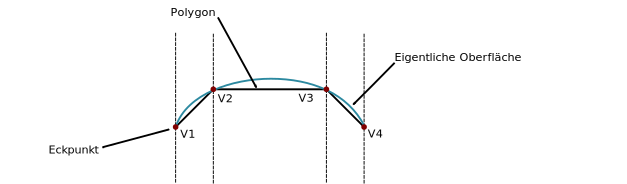
\includegraphics{img/shading_mesh.pdf}
    \caption{Illustration der Ausgangslage\protect\footnotemark}\label{
        fig:shading_mesh_illustration}
\end{figure}
\footnotetext{Eigene Darstellung mittels Inkscape, angelehnt
    an~\cite{hughes_computer_2013}}

Um die Intensität der Farbe für einen Eckpunkt $\bm{V}_{1}$ zu
berechnen, wird der Normalenvektor des Eckpunktes (\textit{vertex
    normal}) benötigt. Es handelt sich dabei um den Normalenvektor der
Oberfläche $\bm{N}$ an der Position des Eckpunktes $\bm{V}_{1}$.

Im Laufe der Zeit hat sich die Schattierung so weit entwickelt, dass
diese praktisch ausschliesslich auf der Grafikkarte (GPU) statt findet.
Man spricht hier vom Begriff ``Shader''. Es handelt sich dabei
mittlerweile um eigene (Grafik-) Applikationen, deren Zweck weit über
die reine Berechnung von Schattierungen hinausgeht.  Man unterscheidet
dabei zwischen Shadern für geometrische Berechnungen (\textit{geometry
    shaders} oder \textit{vertex shaders}) sowie Shader für Berechnungen
bezüglich Pixeln  oder (Bild-) Fragmenten (\textit{pixel shaders} oder
\textit{fragment shaders})~\parencite[Kapitel 33]{hughes_computer_2013}.

Der interessierte Leser sei für weitere Details auf~\cite[Kapitel
33]{hughes_computer_2013},~\cite{opengl_foundation_rendering_2015},
sowie~\cite{fernando_cg_2003} verwiesen.

\subsection{Flat-Shading --- per vertex lighting}
\label{subsec:flat_shading}

% * Calculate normal for each vertice by averaging line-segment normals, e.g.
%   (normal(V1V2) + normal(V3V4)) / 2 to determine per vertex color
%   * Image of calculated normals: line-segment (given through mesh) and vertex
% * One color per face determined by vertex' color

Bei Flat-Shading wird pro Oberfläche (Polygon) ein Eckpunkt $\bm{V}_{1}$
als Schlüssel-Punkt für die Farbe bzw.\ die Intensität bestimmt.  Danach
wird die Farbe des Punktes als Farbe für die gesamte Oberfläche
angenommen~\parencite[S. 734]{foley_computer_1996}.

Diese Annahme ist unter den folgenden Voraussetzungen gültig~\parencite[S. 734]{foley_computer_1996}:
\begin{enumerate}
    \item{Die zugrundeliegende Lichtquelle befindet sich unendlich weit
            entfernt, so dass der Winkel zwischen dem Normalenvektor der
            Oberfläche $\bm{n}$ und der Lichtquelle $\bm{l}$, also
            $\bm{n}\cdot{}\bm{l}$, für die gesamte Oberfläche konstant
            ist.}
    \item{Der Betrachter sich unendlich weit entfernt von der Oberfläche
            befindet, so dass der Winkel zwischen dem Normalenvektor der
            Oberfläche und dem Betrachter $\bm{n}\cdot{}\bm{v}$ für die
            gesamte Oberfläche konstant ist.}
    \item{Das Polygon ist eine effektive Repräsentation der Oberfläche
            und nicht nur eine Näherung einer runden Oberfläche.}
\end{enumerate}

\begin{figure}[H]
    \centering
    
\includegraphics{img/flat_shading.pdf}
    \caption{Illustration des Flat-Shadings\protect\footnotemark}\label{
        fig:flat_shading_illustration}
\end{figure}
\footnotetext{Eigene Darstellung mittels Inkscape, angelehnt
    an~\cite{hughes_computer_2013}}

Ist eine der ersten beiden Annahmen falsch, so muss für den Vektor der
Lichtquelle $\bm{l}$ bzw.\ den Vektor des Betrachters $\bm{v}$ ein
konstanter Wert berechnet werden.~\citeauthor{foley_computer_1996} gibt
hier als Beispiele das Zentrum des Polygones oder den ersten Eckpunkt
des Polygones an~\parencite[S. 735]{foley_computer_1996}.

\subsection{Gouraud-Shading --- face interpolated lighting}
\label{subsec:gouraud_shading}

Bei Gouraud-Shading handelt es sich um ein Shading-Verfahren, welches
die Intensität der Farbe der Eckpunkte von Oberflächen eines Meshes
interpoliert.

\begin{figure}[H]
    \centering
    \includegraphics{img/gouraud_shading.pdf}
    \caption{Illustration des Gouraud-Shadings\protect\footnotemark.}\label{
        fig:gouraud_shading_illustration}
\end{figure}
\footnotetext{Eigene Darstellung mittels Inkscape, angelehnt
    an~\cite{hughes_computer_2013}}

Um die Farbe eines Eckpunktes von Oberflächen zu berechnen,
schlägt~\citeauthor{gouraud_continous_1971} in seiner
Arbeit~\citetitle{gouraud_continous_1971}
von~\citeyear{gouraud_continous_1971} die Berechnung des
Durchschnittswertes der Normalenvektoren der Oberflächen zweier
adjazenter Liniensegmente (im 2D-Raum) bzw.\  aller adjazenter Dreiecke
(im 3D-Raum) vor.

\begin{figure}[H]
    \centering
    \includegraphics{img/shading_mesh_normals.pdf}
    \caption{Illustration der berechneten Normalenvektoren $\bm{n}_{v_{2}}$ und
    $\bm{n}_{v_{3}}$ an den Eckpunkten $v_{2}$ und $v_{3}$ sowie des
    Normalenvektors $\bm{n}_{v_{23}}$ der Kante $\bm{v_{2}v_{3}}$
    \protect\footnotemark.}\label{fig:gouraud_shading_normals_illustration}
\end{figure}
\footnotetext{Eigene Darstellung mittels Inkscape, angelehnt
    an~\cite{hughes_computer_2013}}

Die Berechnung des Normalenvektors eines Eckpunktes via Durchschnittswert ist
üblicherweise eine genügend gute Näherung an die Oberflächennormale der
eigentlichen Oberfläche. Die Präzision hängt dabei aber klar von der
Granularität des Modelles (Mesh) ab.

\subsection{Phong-Shading --- normal interpolated lighting}
\label{subsec:phong_shading}

Phong-Shading ist eine Verbesserung des Gouraud-Verfahrens und bietet eine
bessere Annäherung an die Schattierung bzw. Darstellung von glatten
Oberflächen. Das Verfahren eignet sich vor allem dann besser, wenn ein
Beleuchtungsmodell verwendet wird, welches kleine spiegelnde Reflexionen
bietet, wie z.B. das Phong-Beleuchtungsmodell.

Bei Phong-Shading wird ein Normalenvektor linear an einer Oberfläche
(eines Polygons) interpoliert, ausgehend von den Normalenvektoren der
Kanten der Oberfläche (im obigen Beispiel wäre dies
$\bm{n}_{v_{2}v_{3}}$). Die Oberflächennormale wird an jedem Pixel
interpoliert und normalisiert und kommt dann für die Berechnung der
Farbwerte anhand eines Beleuchtungsmodelles, wie zum Beispiel das
Phong-Beleuchtungsmodell, zum Einsatz. Daher ist Phong-Shading viel
rechenintensiver als Gouraud-Shading, da das Beleuchtungsmodell für
jeden Pixel anstatt für jede Kante berechnet werden muss.

\begin{figure}[H]
    \centering
    \includegraphics{img/phong_shading_mesh_normals.pdf}
    \caption{Stark vereinfachte Illustration der interpolierten
        Normalenvektoren anhand der Kante $\bm{v_{2}v_{3}}$
    \protect\footnotemark.}\label{fig:phong_shading_normals_illustration}
\end{figure}
\footnotetext{Eigene Darstellung mittels Inkscape, angelehnt
    an~\cite{hughes_computer_2013}}

\begin{table}[H]
    \centering
    \caption{Vergleich der genannten Shading-Verfahren anhand einer
    Beispielszene\protect\footnotemark.}\label{table:shading_comparision}
    \begin{tabular}{p{0.2\textwidth}p{0.2\textwidth}p{0.2\textwidth}p{0.2\textwidth}}
        \toprule
            \textbf{Flat-Shading} &
            \textbf{Gouraud-Shading} &
            \textbf{Gouraud-Shading mit Phong-Beleuchtungsmodell} &
            \textbf{Phong-Shading mit Phong-Beleuchtungsmodell} \\
            \cmidrule(r){1-1}\cmidrule(lr){2-2}\cmidrule(lr){3-3}\cmidrule(l){4-4}
            \includegraphics[width=0.2\textwidth]{img/flat_shading_example.pdf} \newline &
            \includegraphics[width=0.2\textwidth]{img/gouraud_shading_example.pdf} \newline &
            \includegraphics[width=0.2\textwidth]{img/phong_gouraud_shading_example.pdf} \newline &
            \includegraphics[width=0.2\textwidth]{img/phong_phong_shading_example.pdf} \newline \\
        \bottomrule
    \end{tabular}
\end{table}
\footnotetext{\cite{brian_danchilla_beginning_2014}}

